\section{Benchmark Test Functions}
Python codes for the test functions discussed under this heading can be accessed through the \href{https://github.com/btayfur/structural-optimization/blob/main/Code/Sources/OptimizationBenchmarks}{link}. \sidenote{
    
\qrcode[height=1in]{https://github.com/btayfur/structural-optimization/blob/main/Code/Sources/OptimizationBenchmarks}}

Standard test functions used to evaluate and compare the performance of optimization algorithms\sidenote{Test functions play an important role in revealing the strengths and weaknesses of algorithms. An algorithm's success in real-world problems is first evaluated on these test functions.} appear as mathematical structures with different difficulty levels. These test functions are designed to challenge algorithms with their known global minimum points, complex local minimum structures, and various topological features.

\subsection{Role of Benchmark Functions in Optimization}

Standard test functions are used to evaluate the performance of optimization algorithms. These functions are important from the following perspectives:

\begin{itemize}
    \item \textbf{Comparability:} Enables objective evaluation of different algorithms' success on the same problem.
    \item \textbf{Identifying Strengths and Weaknesses:} Shows which types of problems algorithms perform well on and which they struggle with.
    \item \textbf{Algorithm Development:} Guides the development and improvement of new optimization algorithms.
    \item \textbf{Preparation for Real-World Applications:} Ensures algorithms are tested before being applied to more complex real-world problems.
\end{itemize}

An ideal benchmark function should reflect the complexity of real-world optimization problems while being mathematically understandable and analyzable. Benchmark functions are generally classified according to the following characteristics: linearity, modality (number of peaks), continuity, differentiability, boundedness, and dimensionality.

\subsubsection{Common Characteristics of Benchmark Functions}

Most benchmark functions have the following characteristics:

\begin{itemize}
    \item Known global minimum value and location
    \item Mathematically defined structure
    \item Adjustable dimension (usually extendable to multidimensional spaces)
    \item Various challenges (e.g., local minima, flat regions, steep valleys)
    \item Recommended search ranges
\end{itemize}

\subsection{Multimodal and Unimodal Test Functions}

Test functions are divided into two categories based on the number of peaks (modes) they contain: unimodal and multimodal.

\subsubsection{Unimodal Functions}

Unimodal functions have only one global minimum and are generally simpler in structure. These functions are used to test the convergence speed and precision of algorithms. Examples include:

\begin{itemize}
    \item \textbf{Sphere Function:} The mathematically simplest optimization test function, defined as:
    \begin{equation}
        f(\mathbf{x}) = \sum_{i=1}^{n} x_i^2
    \end{equation}
    Global minimum $f(\mathbf{x}^*) = 0$ is located at $\mathbf{x}^* = (0, 0, \ldots, 0)$.
    
    \item \textbf{Booth Function:} A two-dimensional, bowl-shaped function:
    \begin{equation}
        f(x, y) = (x + 2y - 7)^2 + (2x + y - 5)^2
    \end{equation}
    Global minimum is at $f(1, 3) = 0$.
\end{itemize}

\subsubsection{Multimodal Functions}

Multimodal functions have multiple local minima and thus test algorithms' ability to find the global minimum without getting stuck in local minima. These functions are particularly important for evaluating the performance of metaheuristic and evolutionary algorithms. Important examples include:

\begin{itemize}
    \item \textbf{Ackley Function:} A complex test function with many local minima. Mathematically defined as:
    \begin{equation}
        f(\mathbf{x}) = -20\exp\left(-0.2\sqrt{\frac{1}{n}\sum_{i=1}^{n}x_i^2}\right) - \exp\left(\frac{1}{n}\sum_{i=1}^{n}\cos(2\pi x_i)\right) + 20 + e
    \end{equation}
    
    This function's global minimum is $f(\mathbf{x}^*) = 0$ at $\mathbf{x}^* = (0, 0, \ldots, 0)$. It is typically defined in the range $[-32.768, 32.768]$.
    
    \item \textbf{Rastrigin Function:} A challenging function with many local minima due to sinusoidal modulation:
    \begin{equation}
        f(\mathbf{x}) = 10n + \sum_{i=1}^{n} \left[ x_i^2 - 10\cos(2\pi x_i) \right]
    \end{equation}
    Global minimum is $f(\mathbf{x}^*) = 0$ at $\mathbf{x}^* = (0, 0, \ldots, 0)$.
\end{itemize}

\begin{figure}[h]
    \centering
    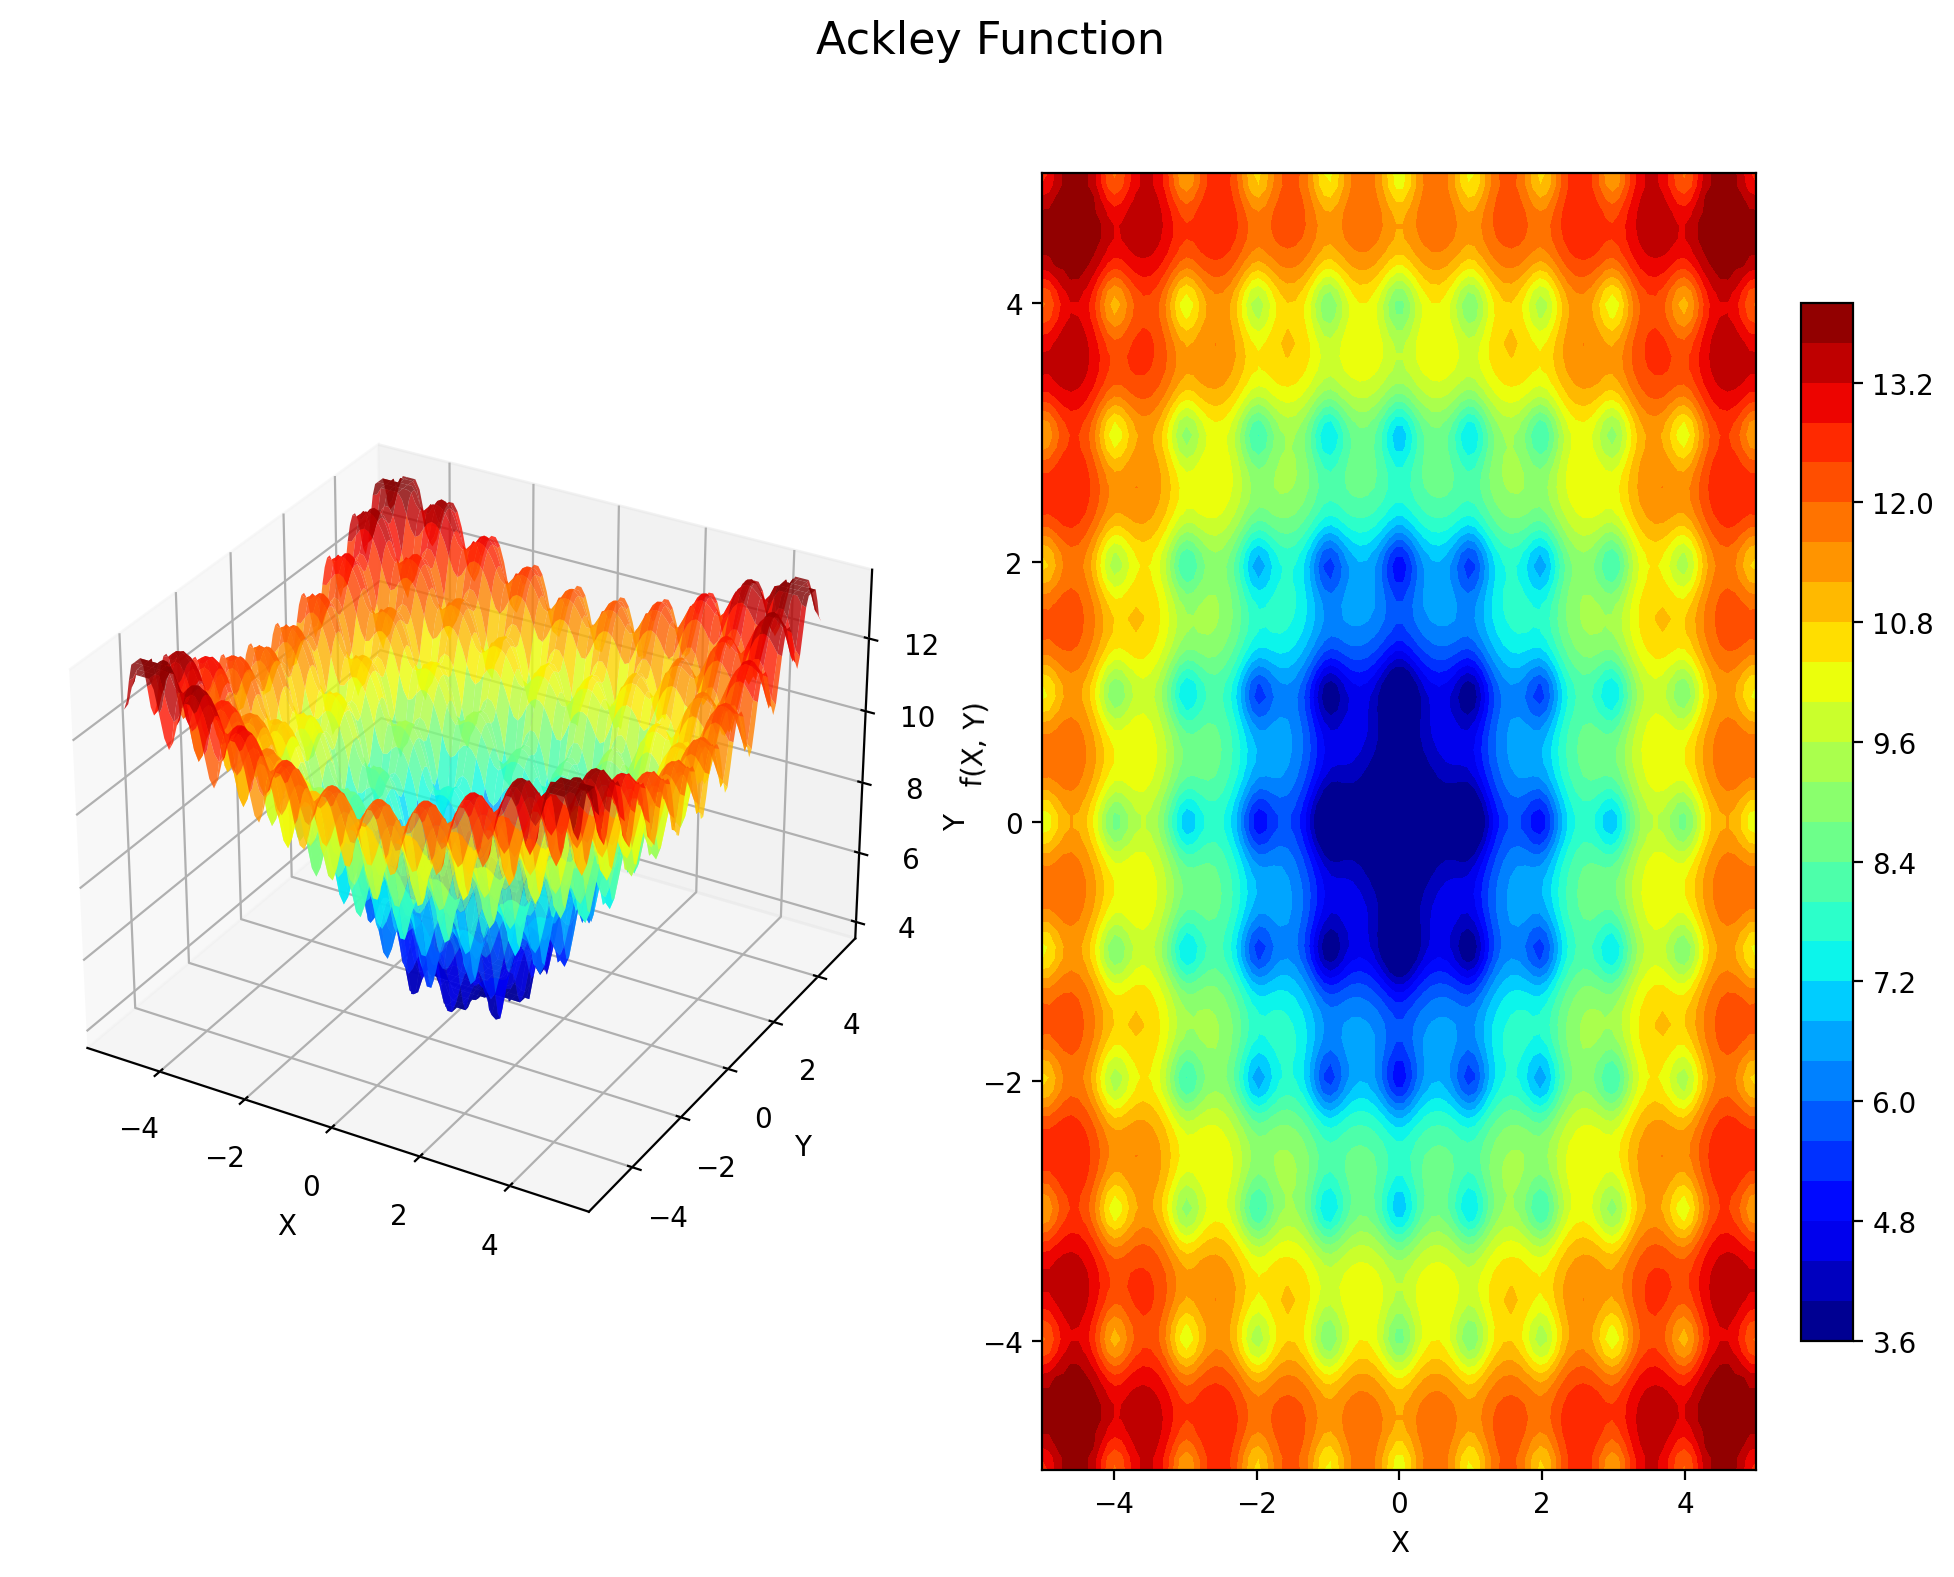
\includegraphics[width=0.8\textwidth]{weeks_new/imgs/ackley_function.png}
    \caption{3D visualization of the Ackley function (left) and contour plot (right). The function's structure with a global minimum at the center and numerous local minima around it is notable.}
    \label{fig:ackley}
\end{figure}

\subsubsection{Ackley Function: In-Depth Analysis}

The Ackley function, proposed by David Ackley in 1987, has become a standard test function for optimization algorithms. The function's mathematical structure reveals the following characteristics:

\begin{itemize}
    \item \textbf{Nearly flat regions:} As we move away from the center, the function has an almost flat structure, making it difficult for gradient-based methods to determine the correct direction.
    
    \item \textbf{Periodic fluctuations:} Due to the cosine term, the function surface shows regular ups and downs, creating many local minima.
    
    \item \textbf{Deep well at the center:} There is a steep well around the global minimum, requiring the algorithm to take precise steps when close to the optimum.
\end{itemize}

The Ackley function is particularly effective in testing the following types of algorithms:

\begin{itemize}
    \item Metaheuristic algorithms that balance local search with global search strategies
    \item Algorithms capable of escaping from numerous local minima
    \item Population-based algorithms that can explore different solution regions simultaneously
\end{itemize}

The optimization of the $n$-dimensional Ackley function involves the following challenges:
\begin{itemize}
    \item The number of local minima increases exponentially with dimension
    \item High precision is required in regions close to the center
    \item Gradient information becomes insufficient in flat regions
\end{itemize}

\begin{tcolorbox}[title=Ackley Function Optimization Challenge]
The Ackley function tests both exploration and exploitation characteristics simultaneously:
\begin{itemize}
    \item Exploration: Finding the correct direction in wide, nearly flat regions
    \item Exploitation: Making precise adjustments in the steep well at the center
    \item Balance: Being able to converge to the global minimum while escaping local minima
\end{itemize}
\end{tcolorbox}

\subsection{High-Dimensional Optimization Problems}

\subsubsection{Effects of Dimension Increase}
\begin{itemize}
    \item Search space grows exponentially
    \item Computational cost increases
    \item Number of local minima increases
    \item Convergence becomes more difficult
\end{itemize}

High-dimensional optimization problems appear in many real-world engineering applications. The increase in dimension leads to the phenomenon known as the "curse of dimensionality." This phenomenon is characterized by the exponential growth of the search space and dramatic decrease in algorithm effectiveness as dimension increases.

\subsubsection{Effects of the Curse of Dimensionality}

The effects of dimension increase on the optimization process:

\begin{itemize}
    \item \textbf{Search space width:} In a problem with $n$ dimensions and $m$ discrete points in each dimension, the total search space is of size $m^n$. For example, with 10 points in each dimension, a 2D problem has 100 points, a 10D problem has $10^{10}$ points, and a 100D problem has $10^{100}$ points.
    
    \item \textbf{Data sparsity:} In high dimensions, distances between data points increase and data becomes sparse. This makes it difficult for algorithms to determine the correct direction.
    
    \item \textbf{Sampling difficulty:} The number of points needed to sufficiently sample high-dimensional space is impractically large.
\end{itemize}

\subsubsection{High-Dimensional Test Functions}

Some test functions are specifically designed to evaluate algorithms' performance in high-dimensional problems:

\begin{itemize}
    \item \textbf{Rosenbrock Function:} A function that progresses along a narrow valley and becomes more challenging as dimension increases:
    \begin{equation}
        f(\mathbf{x}) = \sum_{i=1}^{n-1} \left[ 100(x_{i+1} - x_i^2)^2 + (x_i - 1)^2 \right]
    \end{equation}
    
    \item \textbf{Schwefel Function:} Has many wide-region local minima in high dimensions:
    \begin{equation}
        f(\mathbf{x}) = 418.9829n - \sum_{i=1}^{n} x_i\sin(\sqrt{|x_i|})
    \end{equation}
\end{itemize}

\subsection{Testing Stochastic Algorithms}

Stochastic algorithms are non-deterministic algorithms with random elements. These algorithms can produce different results each time they are run. Modern optimization methods such as metaheuristic algorithms, evolutionary algorithms, and artificial neural networks typically have stochastic characteristics.

\subsubsection{Testing Principles for Stochastic Algorithms}

\begin{itemize}
    \item \textbf{Multiple runs:} The algorithm should be run multiple times (typically 30-50 independent runs) for each test function.
    
    \item \textbf{Statistical analysis:} The mean, standard deviation, median, best and worst values of the results should be reported.
    
    \item \textbf{Convergence analysis:} The algorithm's behavior over time should be shown with a graph of the best value against iteration/evaluation count.
    
    \item \textbf{Parameter sensitivity:} The algorithm's sensitivity to parameter changes should be tested.
\end{itemize}

\subsection{Testing Principles}

Some basic principles should be followed for fair and comprehensive evaluation of optimization algorithms:

\begin{itemize}
    \item \textbf{Variety:} Test functions with different characteristics should be used.
    
    \item \textbf{Fair comparison:} The same conditions (starting points, function evaluation count, termination criteria) should be provided for all compared algorithms.
    
    \item \textbf{Sufficient repetition:} Sufficient number of independent runs should be performed for stochastic algorithms.
    
    \item \textbf{Dimension variation:} Algorithms' performance at different problem dimensions should be tested.
    
    \item \textbf{Comprehensive reporting:} Not only mean or best values but complete statistical results should be reported.
\end{itemize}

\subsection{Performance Metrics}

The performance of optimization algorithms can be evaluated using various metrics. These metrics can be divided into two main categories: numerical and quality metrics.

\subsubsection{Numerical Metrics}

\begin{itemize}
    \item \textbf{Convergence speed:} Shows how quickly the algorithm reaches the desired solution. Usually measured as function evaluation count or iteration count.
    
    \item \textbf{Precision:} Shows how close the found solution is to the known global optimum. Usually measured as absolute or relative error.
    
    \item \textbf{Success rate:} The percentage of times the algorithm reaches an acceptable solution. Particularly important for stochastic algorithms.
    
    \item \textbf{Computational complexity:} Can be measured as running time or memory usage.
\end{itemize}

\subsubsection{Quality Metrics}

\begin{itemize}
    \item \textbf{Robustness:} The algorithm's sensitivity to different problem types, initial conditions, and parameter changes.
    
    \item \textbf{Generalizability:} The algorithm's performance across different problem classes.
    
    \item \textbf{Scalability:} Changes in algorithm performance as problem dimension increases.
    
    \item \textbf{Exploration-exploitation balance:} The algorithm's ability to balance global search (exploration) and local improvement (exploitation).
\end{itemize}

\sidenote{Performance metrics enable objective comparison of different algorithms. However, evaluating multiple metrics together rather than a single metric is more reliable.}

\begin{tcolorbox}[title=No Free Lunch Theorem]
No optimization algorithm can show the best performance on all problems:
\begin{itemize}
    \item Every algorithm has strengths and weaknesses
    \item Choosing an algorithm suitable for the problem structure is important
    \item Hybrid approaches may be advantageous
\end{itemize}
\end{tcolorbox}

\subsubsection{Presentation of Benchmark Results}

The following methods can be used for effective presentation of benchmark test results:

\begin{itemize}
    \item \textbf{Table format:} Tables showing mean, standard deviation, best and worst values for each test function.
    
    \item \textbf{Convergence graphs:} Graphs showing the change in best value against iteration/evaluation count.
    
    \item \textbf{Box plots:} Visual graphs showing the distribution of results and statistical summaries like median and quartiles.
    
    \item \textbf{Ranking tables:} Tables showing performance rankings of algorithms for each test function.
    
    \item \textbf{Statistical significance tests:} Tests (t-test, Wilcoxon signed-rank test, Friedman test, etc.) showing whether performance differences between algorithms are statistically significant.
\end{itemize}

\subsection{Categories of Benchmark Functions}

Benchmark functions with different characteristics test algorithms' ability to handle various challenges. Here, basic function categories and examples are given:

\subsubsection{Functions with Many Local Minima}

These functions have many local minima that pose a challenge for algorithms and test global optimization ability:

\begin{itemize}
    \item Ackley
    \item Rastrigin
    \item Griewank
    \item Schwefel
    \item Levy
    \item Shubert
\end{itemize}

\subsubsection{Bowl-Shaped Functions}

These functions have a single minimum surrounded by circular or elliptical contours and test local optimization ability:

\begin{itemize}
    \item Sphere
    \item Bohachevsky
    \item Sum Squares
    \item Rotated Hyper-Ellipsoid
\end{itemize}

\subsubsection{Plate-Shaped Functions}

These functions have flat regions that can challenge algorithms' ability to determine the correct direction:

\begin{itemize}
    \item Booth
    \item Matyas
    \item Zakharov
    \item McCormick
\end{itemize}

\subsubsection{Valley-Shaped Functions}

These functions have long, narrow valleys that can slow down the convergence of many algorithms:

\begin{itemize}
    \item Rosenbrock (Banana Function)
    \item Six-Hump Camel
    \item Three-Hump Camel
    \item Dixon-Price
\end{itemize}

\subsubsection{Functions with Steep Ridges/Drops}

These functions have steep ridges or drops that can challenge gradient-based methods:

\begin{itemize}
    \item Easom
    \item Michalewicz
    \item De Jong N.5
\end{itemize}

\subsection{Conclusion and Applications}

Benchmark test functions are indispensable tools for the development, testing, and comparison of optimization algorithms. These functions help evaluate algorithms' performance on different problem types and identify their weaknesses.

\begin{itemize}
    \item \textbf{In algorithm development:} Determining strengths and weaknesses of new algorithms
    \item \textbf{In parameter tuning:} Optimization of algorithm parameters
    \item \textbf{In hybrid approaches:} Development of hybrid methods combining strengths of different algorithms
    \item \textbf{In education:} Understanding the behavior of optimization algorithms
    \item \textbf{In preparation for real-world problems:} Evaluating basic capabilities of algorithms before moving to more complex problems
\end{itemize} 